%% ---------------------------------------------------------------------------
%% intro.tex
%%
%% Introduction
%%
%% $Id: intro.tex 1477 2010-07-28 21:34:43Z palvarado $
%% ---------------------------------------------------------------------------

\chapter{Diagramas de Gantt y PERT}
\label{chp:diagramas}

Se inicia el proyecto con las tareas de investigación. A partir de la investigación se determina qué marco de trabajo utilizar para entrenar el bosque de decisión aleatoria y qué estrategias de extracción de características usar para entrenar el bosque. Luego se diseña e implementa el bosque, cual se espera que dure varias semanas para lograr cumplir con los requisitos de calidad requeridos. Finalmente las tareas de optimización se realizan cuando se termine de entrenar el bosque. El Diagrama de Gantt mostrado en la Figura \ref{fig:gantt} ilustra la distribución de actividades en el tiempo. Además, se resalta la ruta crítica del proyecto. Las tareas se inician a partir del 6 de Febrero y se esperan que vayan concluyendo para la última semana de Abril.

\begin{figure} [!h]
    \centering
    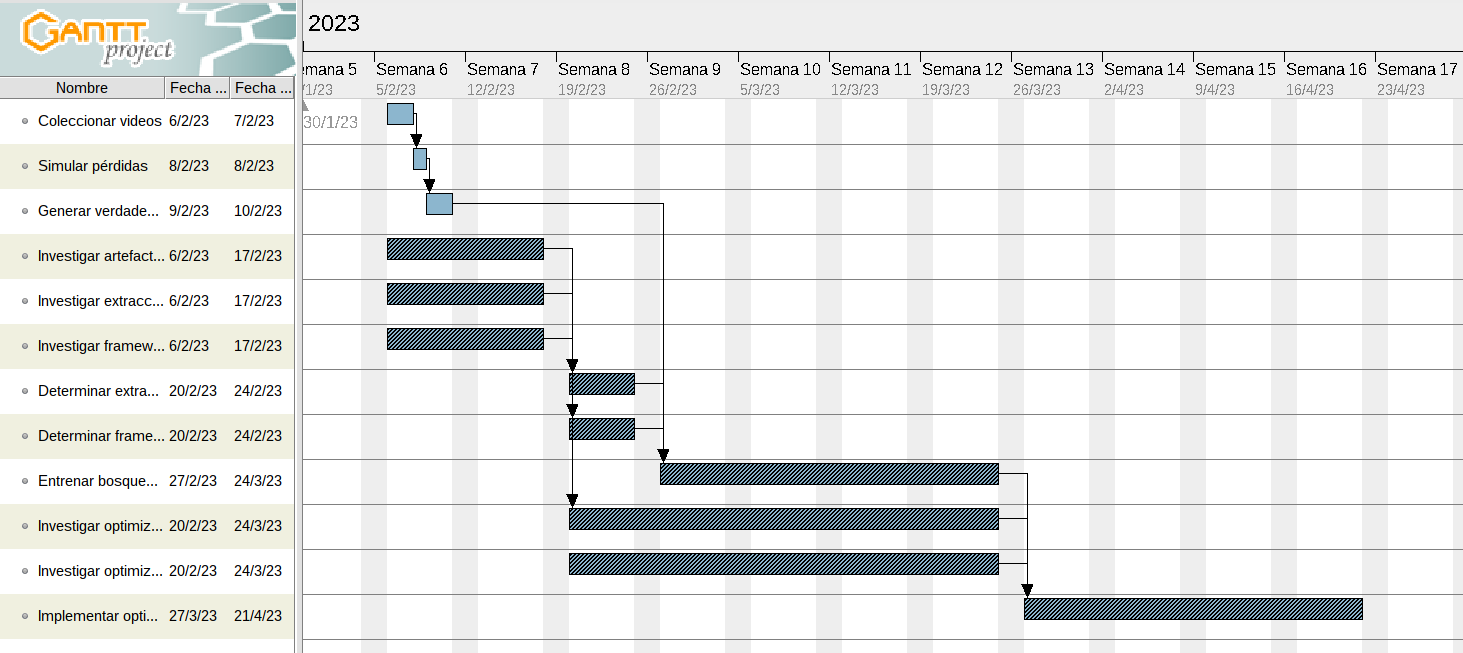
\includegraphics[width=\textwidth]{gantt.png}
    \caption{Diagrama de Gantt}
    \label{fig:gantt}
\end{figure}

El siguiente Diagrama de PERT ilustra la relación de dependencias entre las
actividades a realizar.

\begin{figure} [!htb]
    \centering
    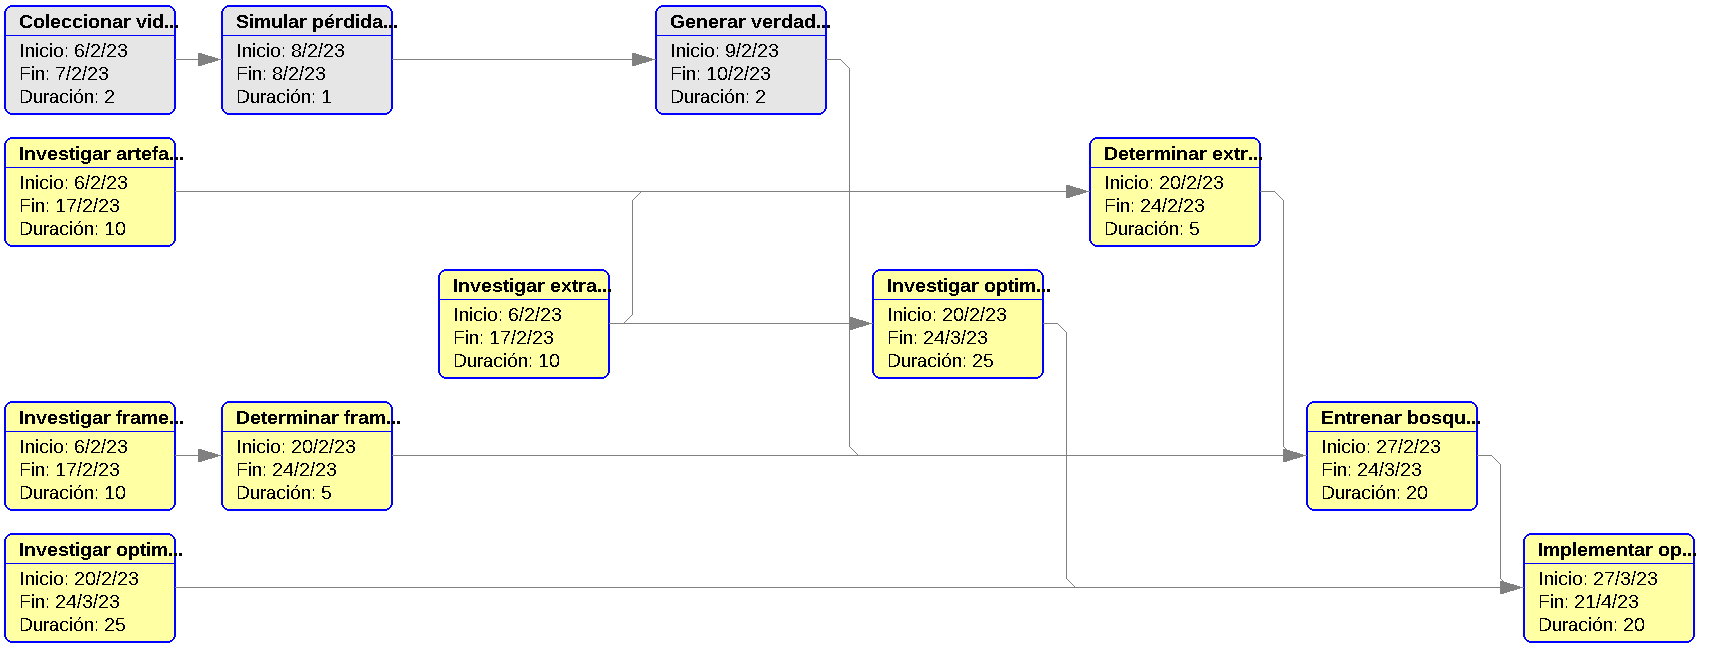
\includegraphics[width=\textwidth]{pert.png}
    \caption{Diagrama de PERT}
    \label{fig:pert}
\end{figure}

El presupuesto del proyecto se muestra en la Figura \ref{fig:presupuesto} y el aporte mensual de la empresa se muestra en la Figura \ref{fig:mensual}.

Como recurso principal del proyecto, se utiliza una de las Nvidia Jetson TX2 del SIPLab de la Escuela de Electrónica del Tec. Para entrenar los modelos, es necesario contar con amplia RAM para lograr cargar los datos de entrenamiento. El Servidor de la Escuela de Electrónica cuenta con una máquina virtual con el sistema operativo Ubuntu 22.04 instalado y 64 Gb de RAM para este propósito. Para el desarrollo de los algoritmos y pruebas, se utiliza una máquina personal.

\begin{figure} [!htb]
    \centering
    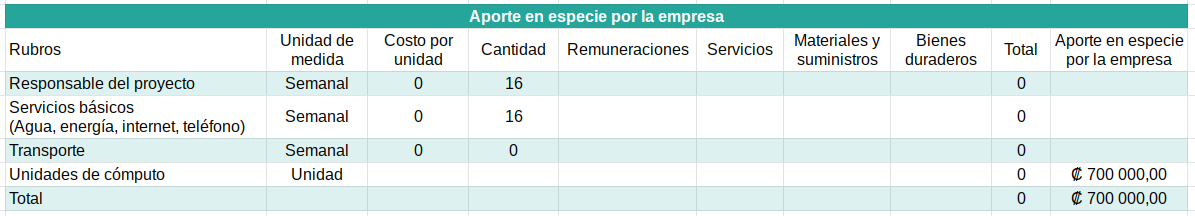
\includegraphics[width=\textwidth]{presupuesto.png}
    \caption{Presupuesto del proyecto}
    \label{fig:presupuesto}
\end{figure}

\begin{figure} [!htb]
    \centering
    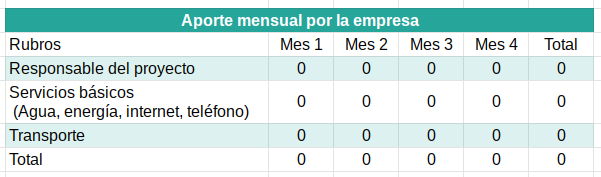
\includegraphics[width=0.5\textwidth]{mensual.png}
    \caption{Aporte mensual de la empresa}
    \label{fig:mensual}
\end{figure}
